\chapter{Results}
\label{chap:3}
\ChapterPageStuff{3}

\section{Introduction}
In \Cref{sec:ch2_preamble} the methodology is created for a web based software system. As describe in this section that a user can have multiple systems and subssyrtems linked to their account. The implementation is done for multiple software systems in this section. The system implementation will focus more on the development of the logging mechanism and the critic analysis will be of the Priortising of software maintenance using a utilisation analysis.

\section{Implementation}
To implement the development of solution that is discussed in \Cref{sec:ch2_developementOfSolution} three different software systems will be used. These systems is created make use of \texttt{APS.NET Core Web SDK} and \texttt{PHP}. Usisng these systems will enable to create a logging mechanism for newer and older software systems.

\subsection{System Implementation}
When working with both \texttt{ASP.NET Core Web SDK} and \texttt{PHP}, there may be similarities and shared system implementations. However, discrepancies may arise between the two technologies, particularly in the area of logging mechanisms. It is important to note the specific implementation and resulting behaviors to effectively troubleshoot any issues that may occur.

\subsubsection{Log attibutes}\label{sec:ch3_logAtrributes}
Using the functional requirements discussed in \Cref{sec:ch2_logAttributesRequirements}

\begin{table}[!htb]
	\centering
	\caption[Logging attributes]
	{\textit{Logging attributes}}
	\label{tbl:ch3_Log_Attributes}
	\begin{tabularx}{\textwidth}{|l|l|X|}
		\hline \textbf{Column name} & \textbf{Requirement ID} & \textbf{Description}\\
		\hline \texttt{laa\_ID} & \ref{fr:lpa1} & User based actvity identifier. \\
		\hline \texttt{laa\_TimeStamp} & \ref{fr:lpa2} & Timesstamp when the activity has occur. \\
		\hline \texttt{laa\_ActivityType} & \ref{fr:lpa3} & Activity type of the log event. \\
		\hline \texttt{fk\_u\_ID} & \ref{fr:lpa4} & Identification number of the user associated with the log event. \\
		\hline \texttt{laa\_Area} & \ref{fr:lpa5} & System where the activity has occur. \\
		\hline \texttt{laa\_Controller} & \ref{fr:lpa5} & Subsystem where the activity has occur. \\
		\hline \texttt{laa\_MetaData} & \ref{fr:lpa6} & Metadata captured from the \textit{HTTP request}. \\
		\hline \texttt{fk\_g\_ID} & \ref{fr:lpa7} & Additional identifiers for the log event. \\
		\hline
	\end{tabularx}
\end{table}

\begin{lstlisting}[style=json, caption={\textit{Metadata JSON}}, label={fig:ch3_MetadataJson}] 
	{
		"RequestOrigin": "/System/Subsystem1/",
		"RequestElementID": "ButtonSaveCsv",
		"RequestParameters": {
			"aTagIDs": [
				"6284",
				"20320"
			],
			"aToDate": "2020-04-06",
			"aGroupID": 2,
			"aFromDate": "2020-03-30"
		}
	}
\end{lstlisting}

\subsubsection{Obtaining the element of user-based event}\label{sec:ch2_ElementObtaining}
In \Cref{sec:ch2_webApplicationArchitecture} the user-based activity event will be use a \textit{HTTP request} to send to the server when the user interacted with an \textit{HTML element}. For the functional requirements activity type (F/R 1.5.3) and metadata (F/R 1.5.6) in \Cref{tbl:ch2_keyLoggingAttributes} the \textit{HTML element} needs to be obtained to get the element's tag and identification text. This can be difficult to obtain due to \textit{bubbling}\footnote{\textbf{Bubbling} is when an event happens on an element, it first runs the handlers on it, then on its parent, then up on other ancestors. \cite{EventBubbling}.} that may occur when searching for the element that the user specifically interacted with.\par In \Cref{fig:ch2_event_bubbling} is the event propagation example of a child element that has been clicked on which executes a DOM event. The event propagation consists of three phases~\cite{EventBubbling}:

\begin{itemize}
	\item \textit{Capturing phase:} The event propagates downwards to the targeted element that the user interacted with.
	\item \textit{Target phase:} The event reaches the targeted element to execute the DOM event.
	\item \textit{Bubbling phase:} The event bubbles up from the targeted element
\end{itemize}

\begin{figure}[!htb] % An h :here, t: top, b: bottom.
	\centering % cent the figure
	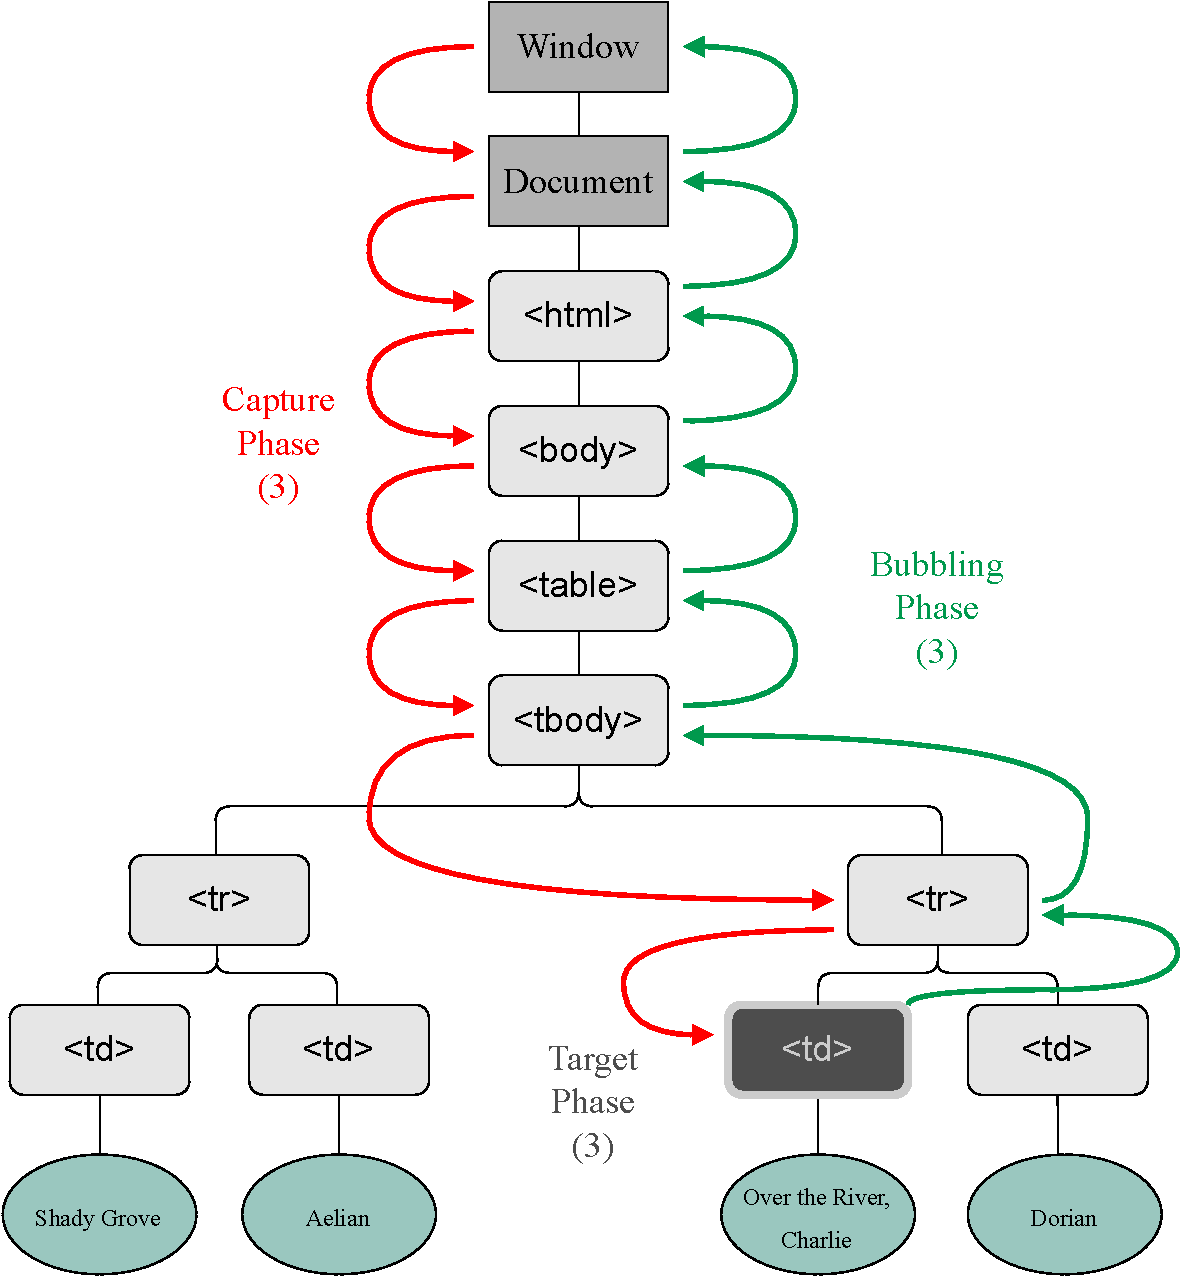
\includegraphics[width=0.6\textwidth]{Chapter2/event_bubbling/event_bubbling.pdf}
	\caption[JavaScript event propagation]
	{\textit{JavaScript event propagation~\cite{EventBubbling}}}\label{fig:ch2_event_bubbling}
\end{figure}

Capturing the targeted element may be difficult as some Web pages may have more complex HTML where the event propagation may sometimes not obtain the correct element information which the user interacted with. Another DOM event may have started during the initial element's event, therefore it is more accurate to obtain the targeted element by obtaining the last known element the user hovered over on the user interface.\par In \Cref{fig:ch2_element_event_capturing} is the flow diagram to capture the element user interacted with for the user-based activity log. This code segment will be initiated during the \texttt{beforeSend} operation of the \textit{AJAX request} to filter HTML elements by predefined allowed elements to use. Filtering the element tag names ensures that unwanted more complex elements or more basic elements that are not expected to be the initiator of the event will be used. \par If the Web location already changed or no element exists, the contents of the page might have already changed during the event propagation. The last known element that the user hovered on must be used as most likely might have been the element that the user interacted with. This will ensure there is always an element that has been detected and parsed with the request header in most UI changes.

\clearpage

\begin{figure}[!htb] % An h :here, t: top, b: bottom.
	\centering % cent the figure
	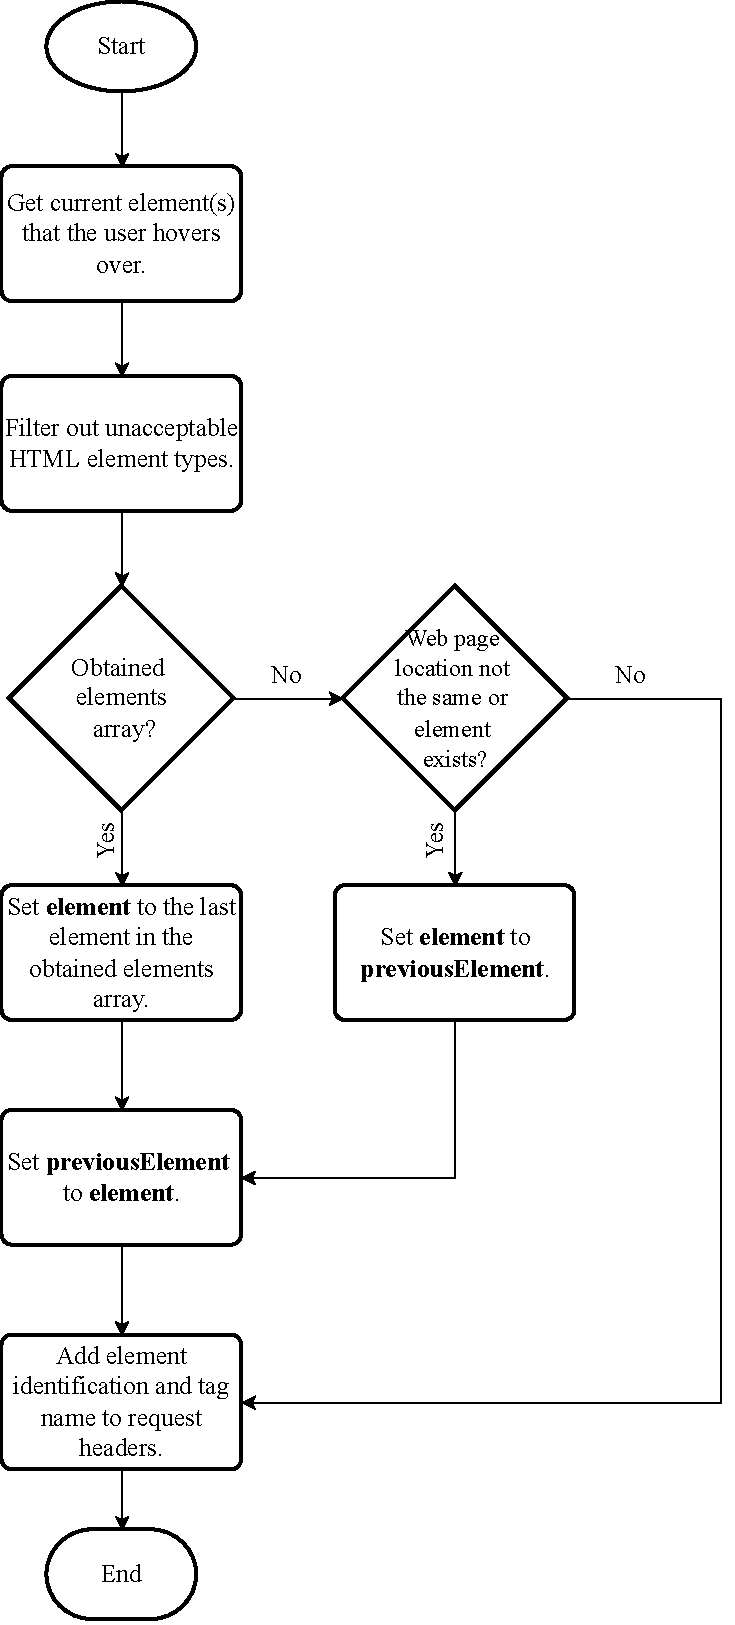
\includegraphics[width=0.5\textwidth]{Chapter2/element_capturing/element_capturing.pdf}
	\caption[HTML element capturing flow diagram]
	{\textit{HTML element capturing flow diagram}}\label{fig:ch2_element_event_capturing}
\end{figure}

\clearpage

\subsubsection{Log attributes}

\section{Case studies}

\subsection{Case study identification}

\subsection{Case study results}

\subsubsection{System A results}

\begin{landscape}
	\begin{figure}[!htb]
		\centering % cent the figure
		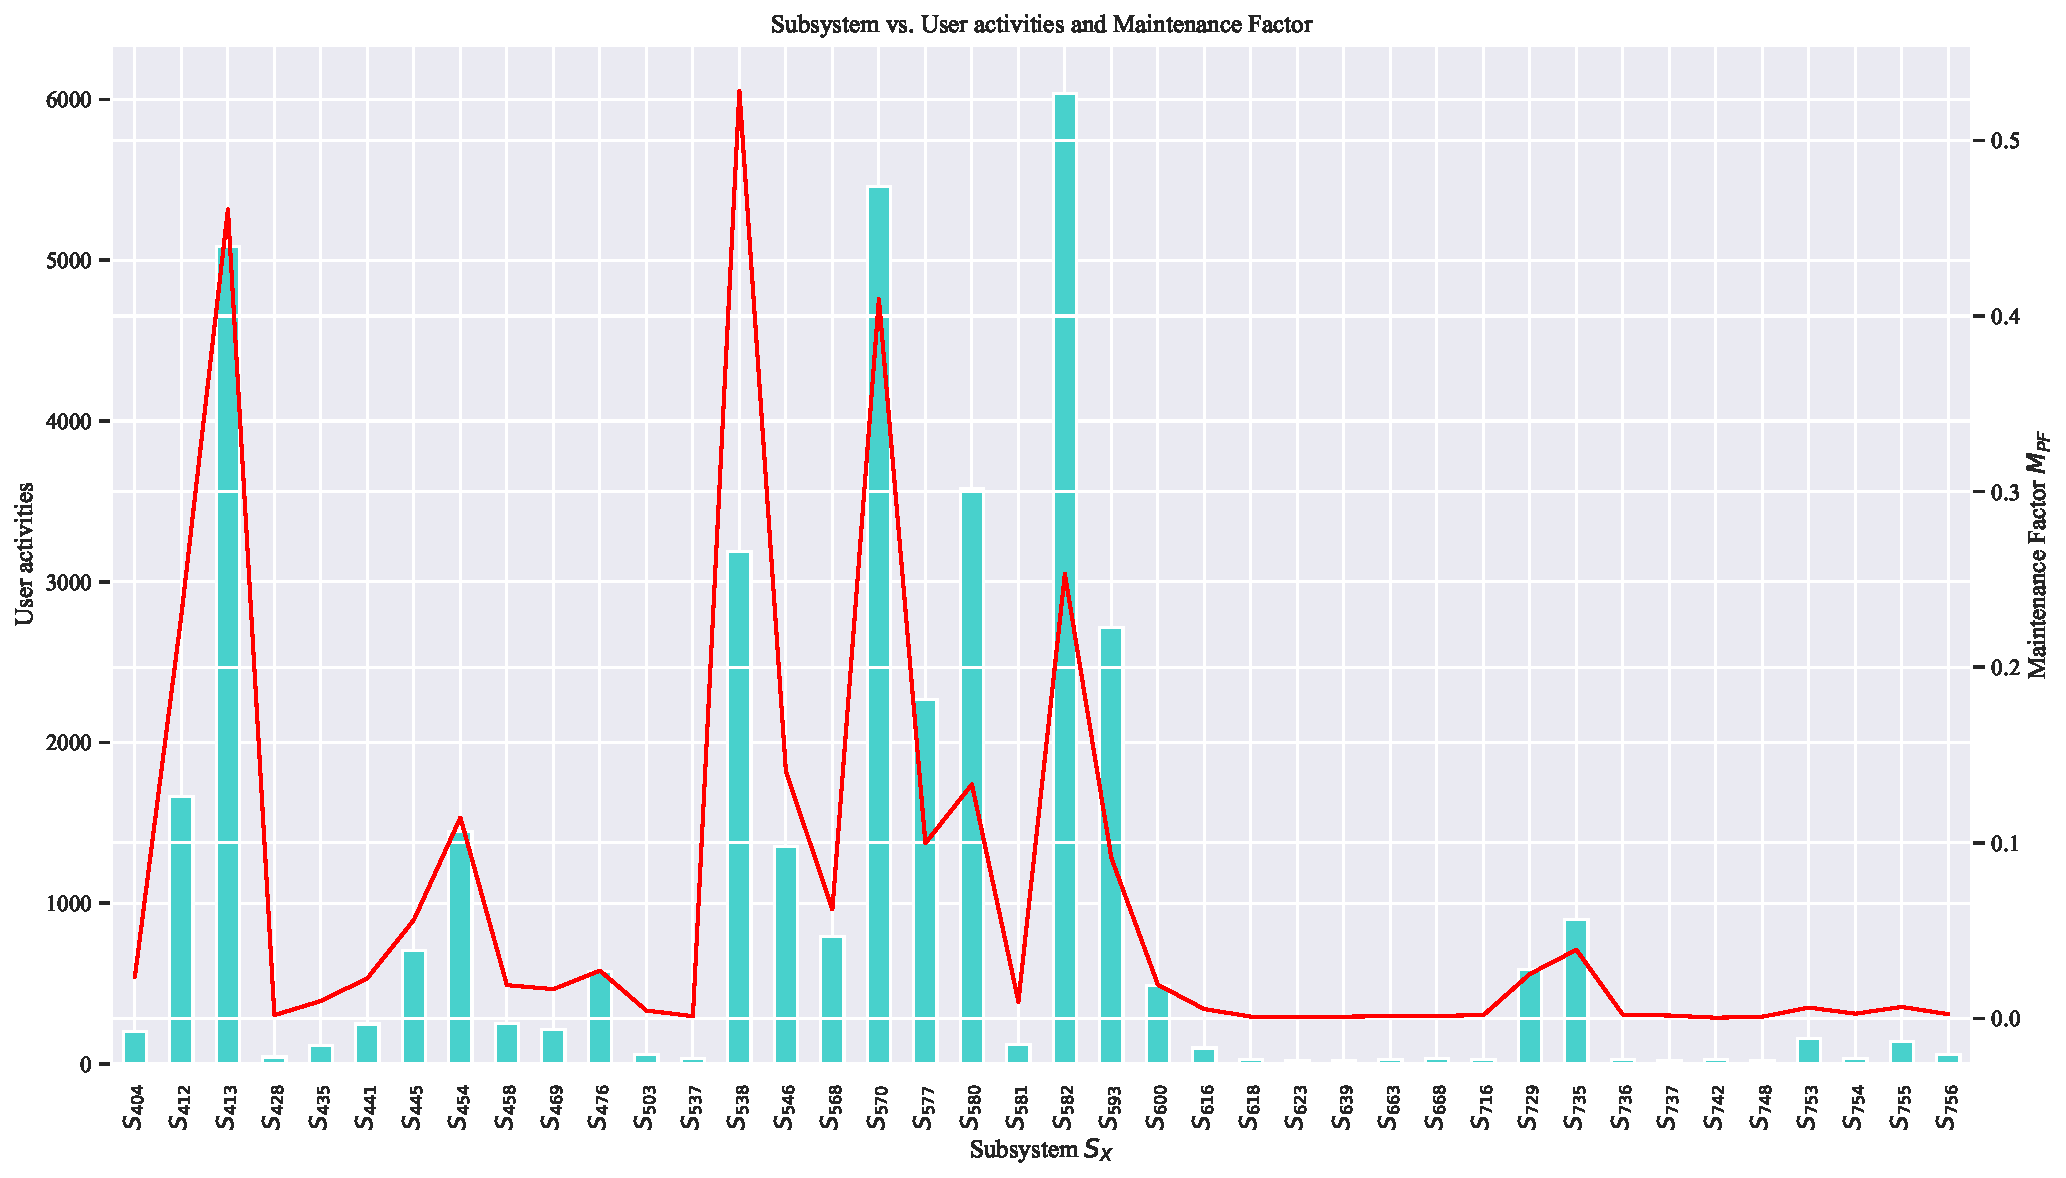
\includegraphics[width=0.95\linewidth]{img/ch3/analysis/case_A_subsystems_1.pdf}
		\caption[Case study 1 subsystem activities part 1]
		{\textit{Case study 1 subsystem activities part 1}}\label{fig:ch3_saS1S24}
	\end{figure} 
\end{landscape}

\subsubsection{System B results}

\begin{landscape}
	\begin{figure}[!htb]
		\centering % cent the figure
		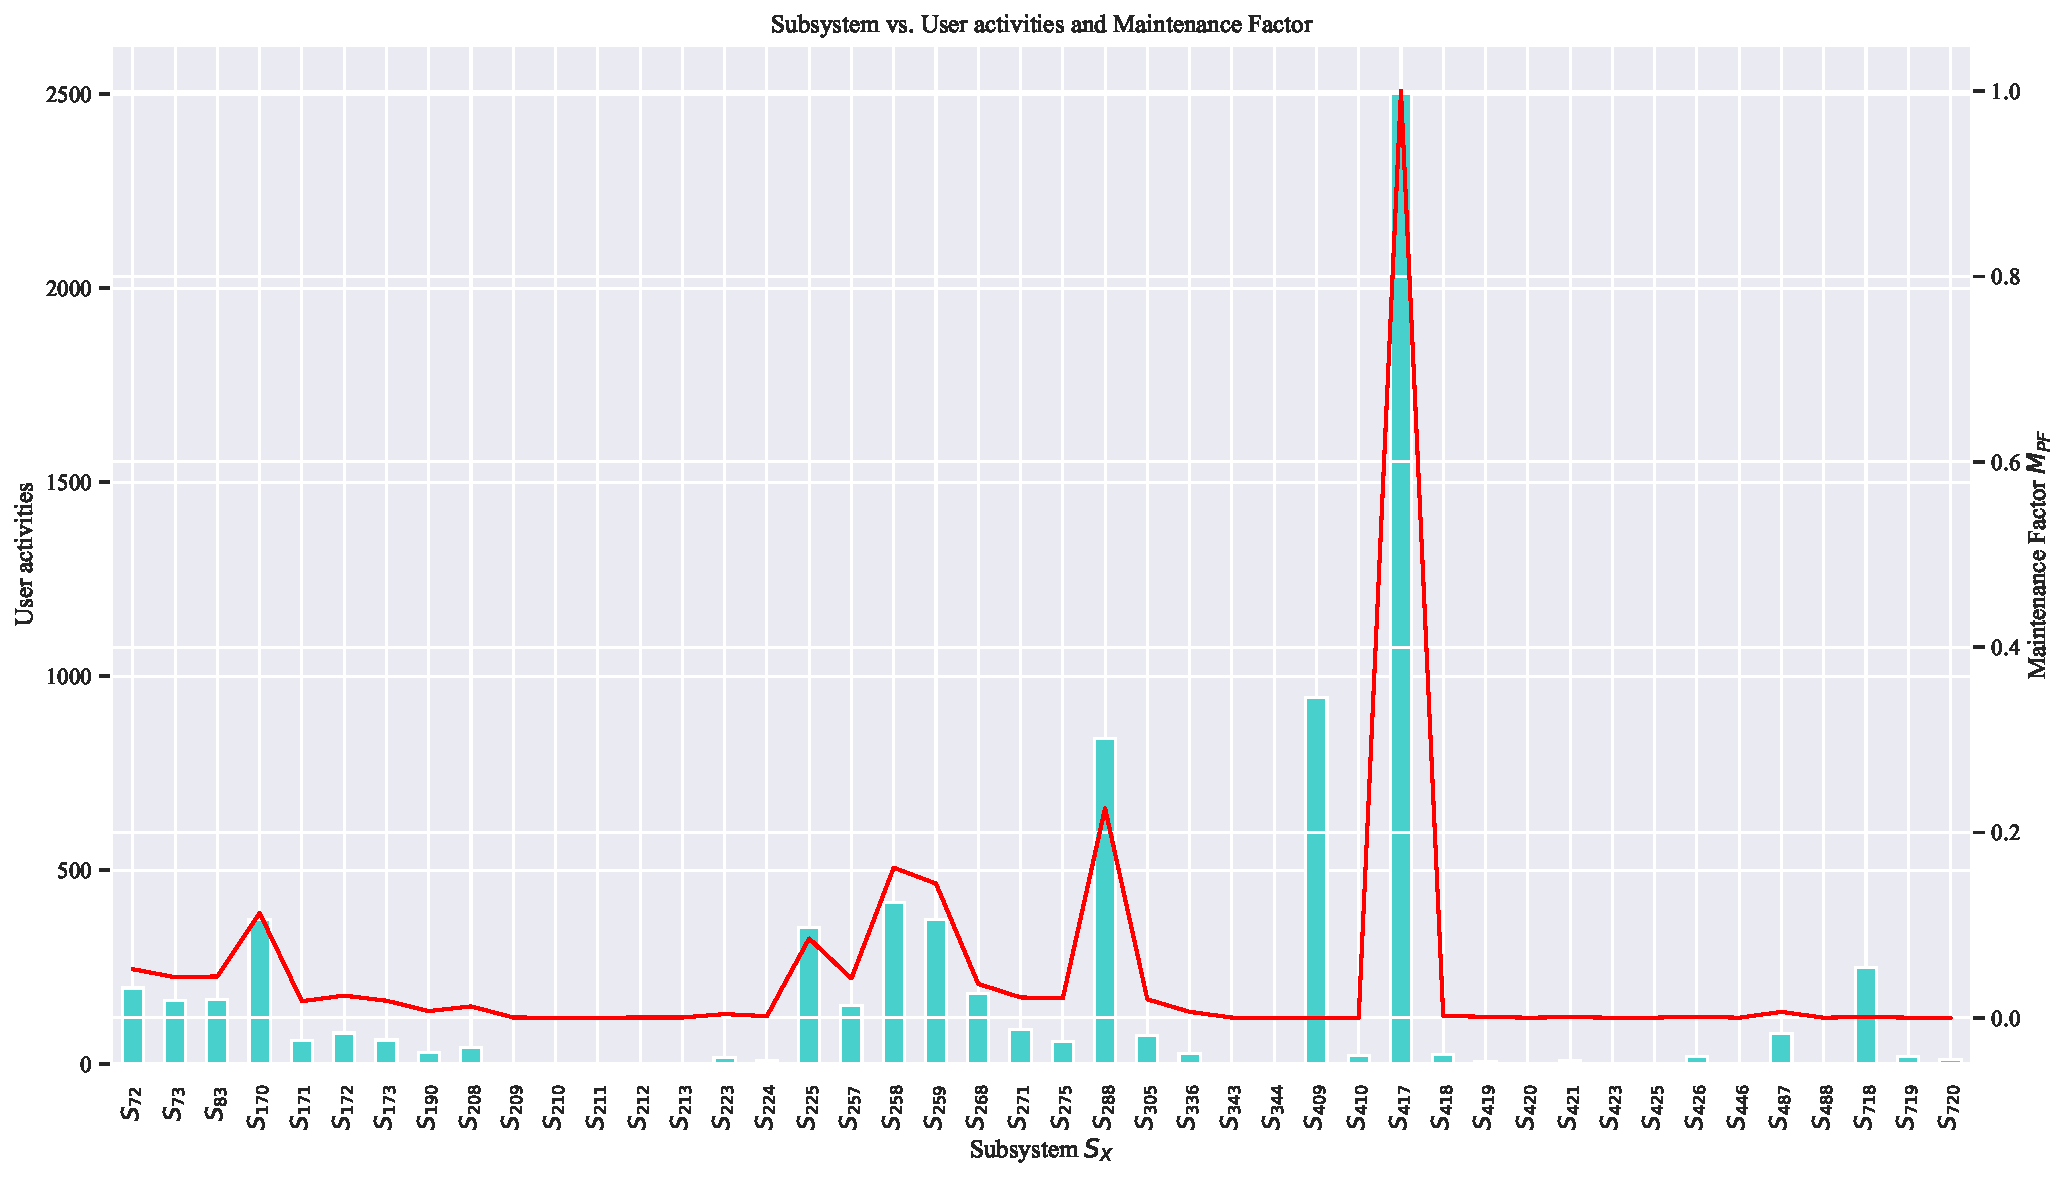
\includegraphics[width=0.95\linewidth]{img/ch3/analysis/case_B_subsystems_1.pdf}
		\caption[Case study 1 subsystem activities part 1]
		{\textit{Case study 1 subsystem activities part 1}}\label{fig:ch3_saS1S24}
	\end{figure} 

	\begin{figure}[!htb]
		\centering % cent the figure
		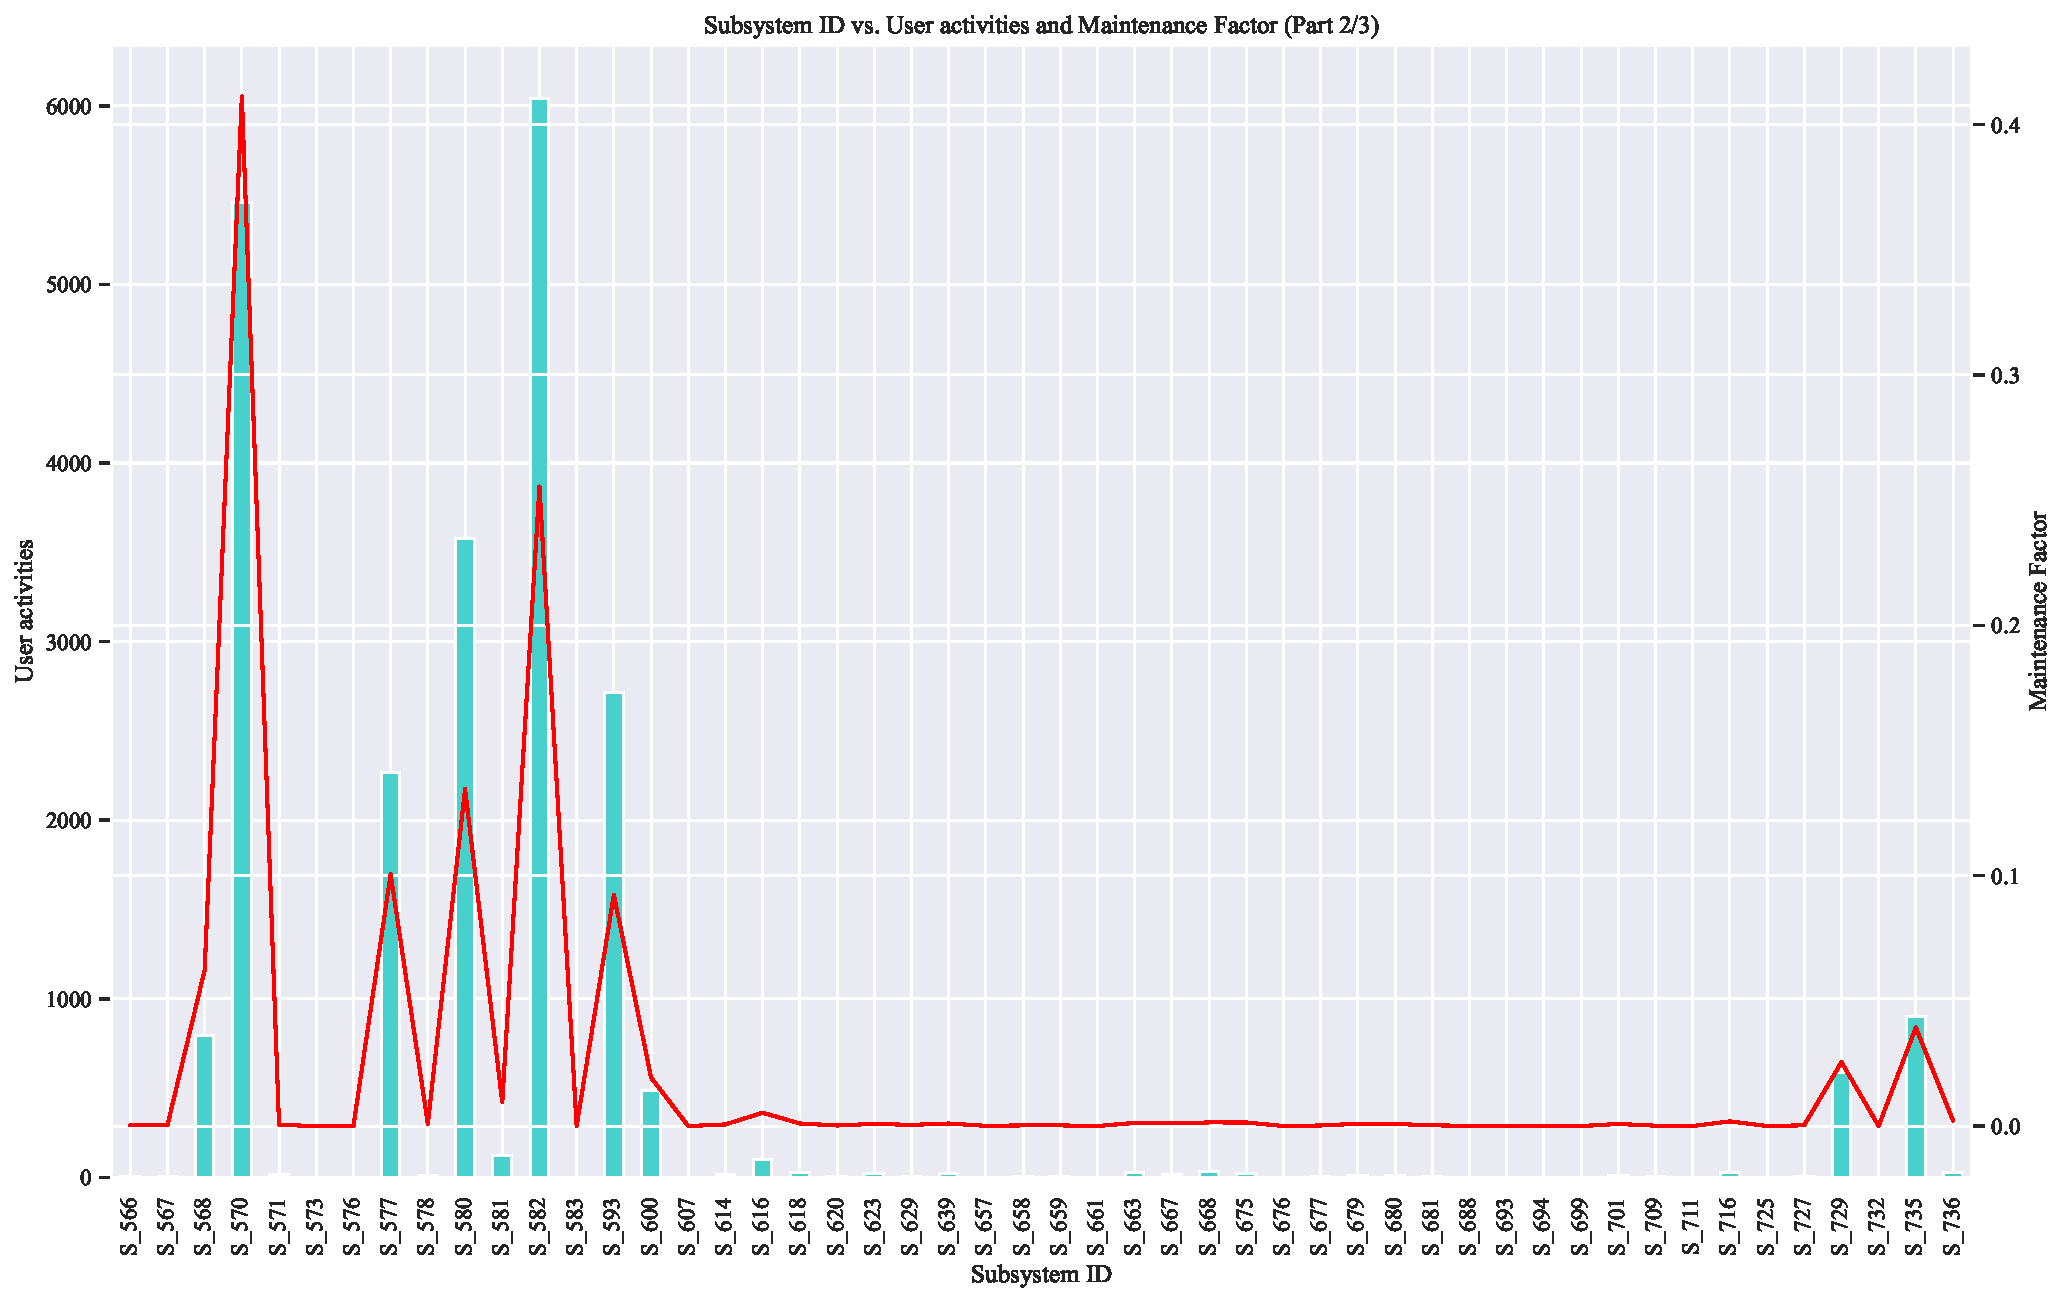
\includegraphics[width=0.95\linewidth]{img/ch3/analysis/case_B_subsystems_2.pdf}
		\caption[Case study 1 subsystem activities part 1]
		{\textit{Case study 1 subsystem activities part 1}}\label{fig:ch3_saS1S25}
	\end{figure} 

	\begin{figure}[!htb]
		\centering % cent the figure
		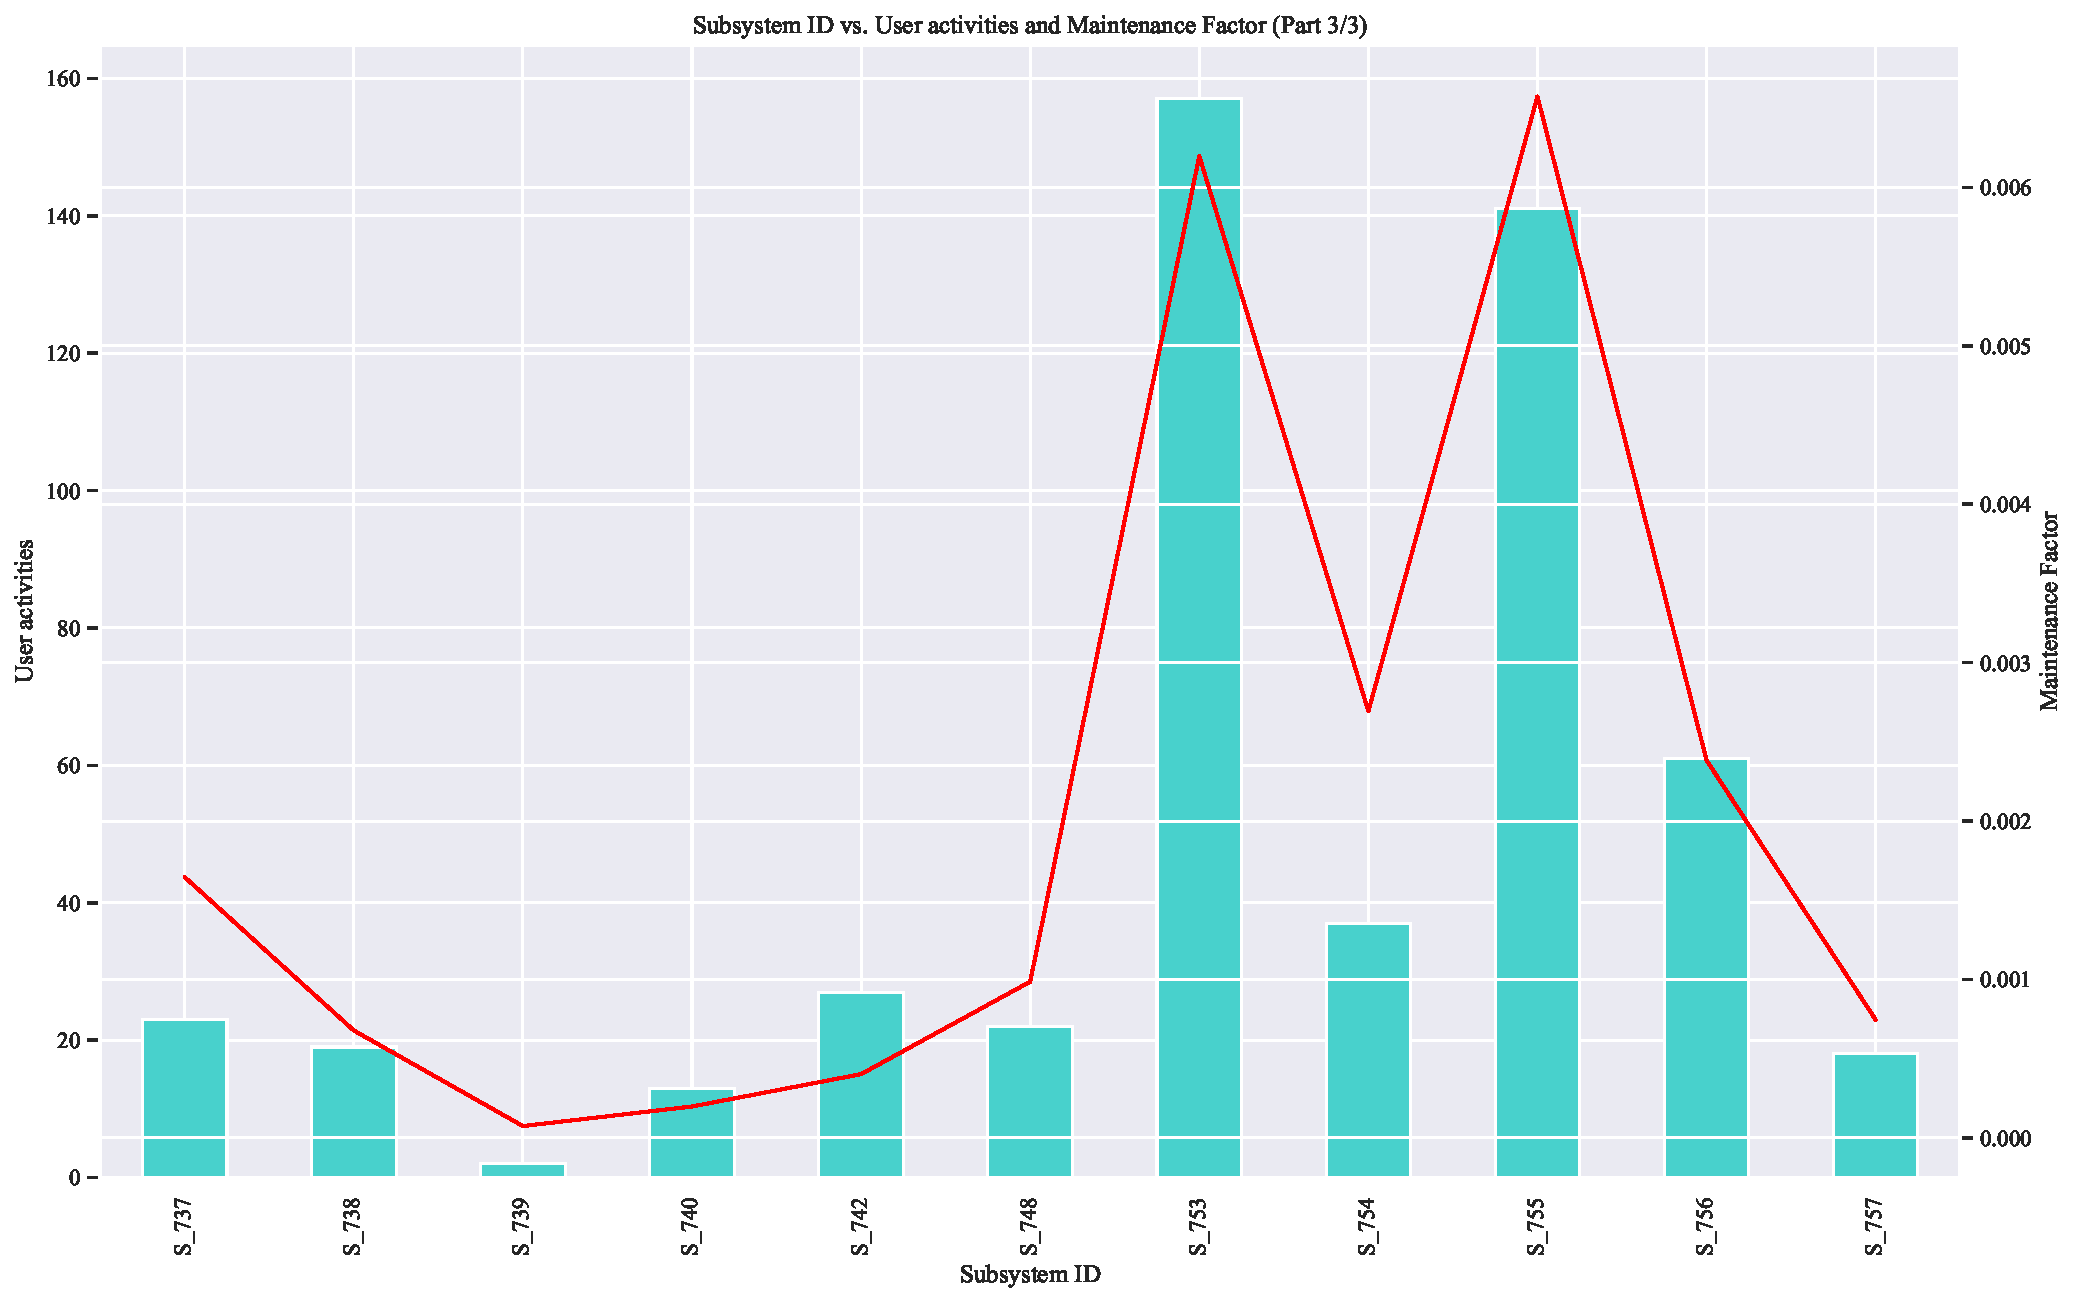
\includegraphics[width=0.95\linewidth]{img/ch3/analysis/case_B_subsystems_3.pdf}
		\caption[Case study 1 subsystem activities part 1]
		{\textit{Case study 1 subsystem activities part 1}}\label{fig:ch3_saS1S26}
	\end{figure} 
\end{landscape}

\clearpage

\subsection{Critical analysis results}

\section{Conclusion}